\level{2}{Interazioni tra classi dei componenti dell'applicazione Android}
	Dopo che sono stati descritte nel dettaglio tutte le varie classi necessarie alla progettazione dell'applicazione \insglo{Android}, è necessario mostrare come le classi appartenenti a componenti differenti interagiscano tra di loro. È quindi inserito in seguito un diagramma \insglo{UML} che rappresenta tutte le interazioni presenti tra i vari componenti.\\
	Si noti che alcune classi non sono state inserite in quanto si è voluto rendere più comprensibile il diagramma.

	\begin{figure}[H]\centering
		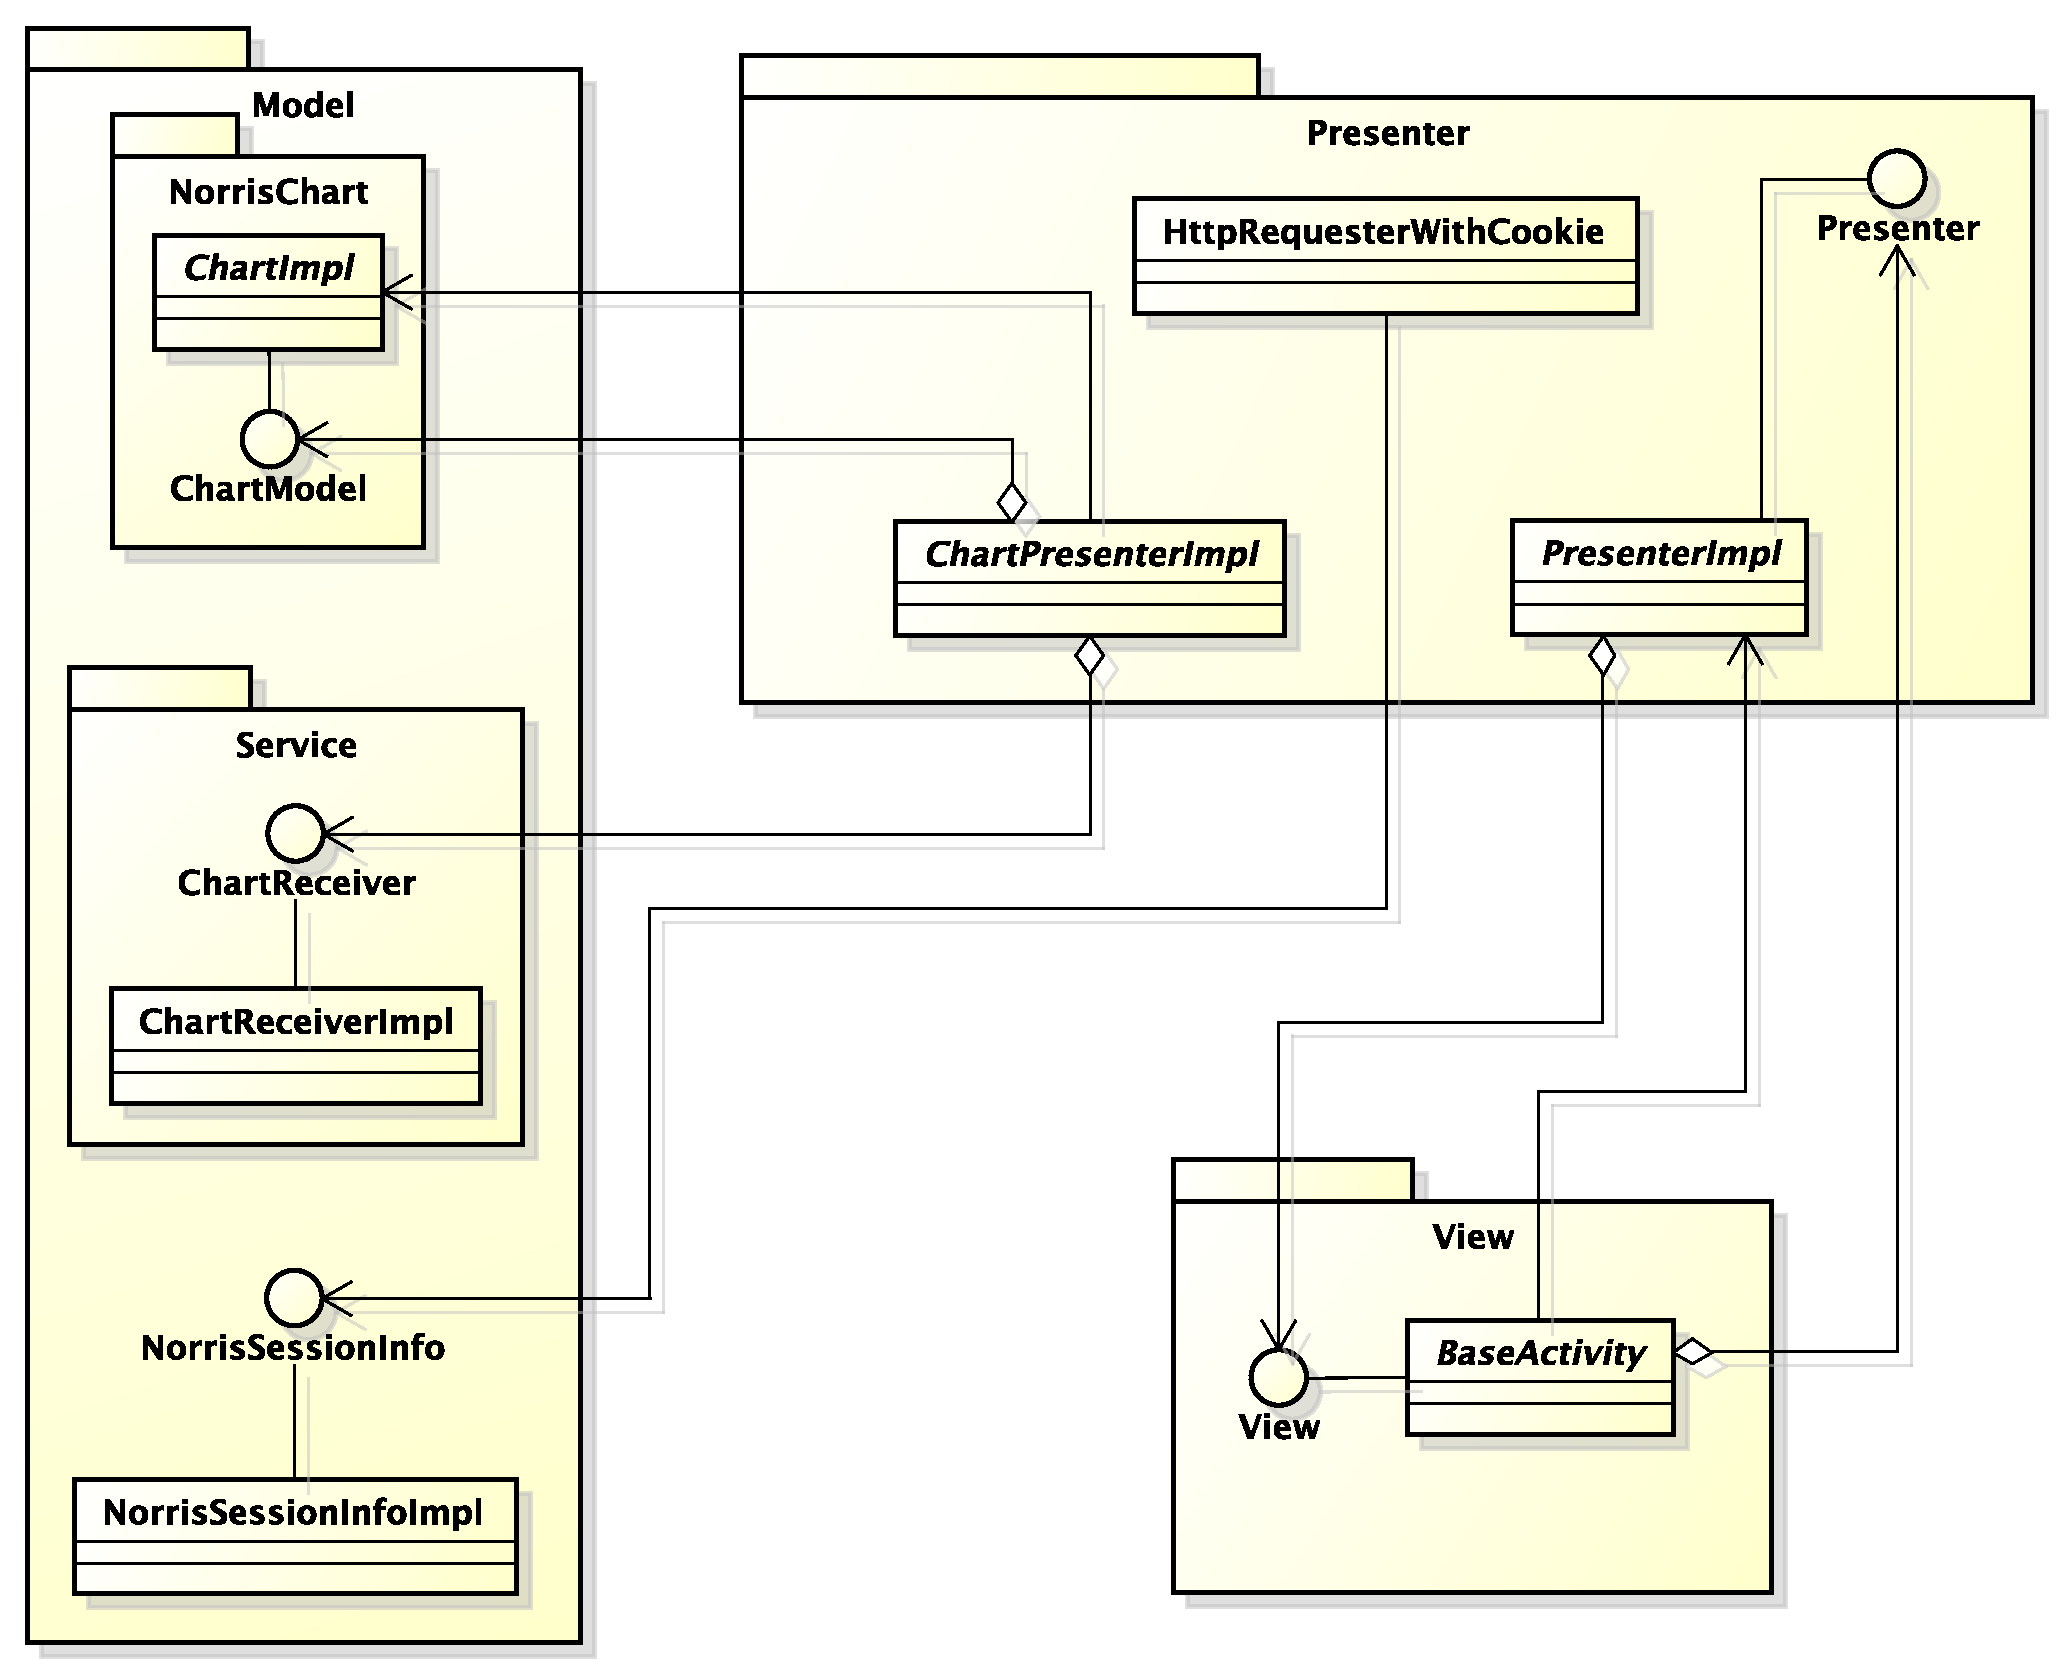
\includegraphics[width=\textwidth]{SpecificaTecnica/Pics/InterazioniComponentiApplicazione.pdf}
		\caption{Diagramma delle interazioni tra classi di componenti dell'Applicazione}
	\end{figure}